\documentclass{jsarticle}
\usepackage{amsmath,amssymb,amscd}
\usepackage[obeyspaces]{url}
\usepackage[all]{xy}
% installed in the system by hand
\usepackage{shuffle}
\usepackage{listings}
\usepackage{float}
\usepackage{sty/simplewick}
\usepackage[enableskew]{sty/youngtab}
\usepackage{sty/jumoline}
\usepackage{sty/boxedminipage}
\usepackage{stmaryrd}
\usepackage{fancybox}
\usepackage{lscape}
%{
\usepackage[dvipdfm,dvips]{color}
\usepackage[dvipdfm,dvips]{graphicx}
\usepackage[dvipdfm %
  , hypertex %
  , colorlinks=true %
  , bookmarks=true %
  , bookmarksnumbered=false %
  , bookmarkstype=toc %
  , pdfkeywords={TeX; dvipdfmx; hyperref; color;} %
	]{hyperref}
\ifnum 42146=\euc"A4A2
  \AtBeginDvi{\special{pdf:tounicode EUC-UCS2}}% platex-utf8 でも OK
\else
  \AtBeginDvi{\special{pdf:tounicode 90ms-RKSJ-UCS2}}%"
\fi
\usepackage{verbatim}
\usepackage{sty/myarrow}
\usepackage{sty/mybraket}
%}
\usepackage[amsmath,hyperref]{sty/ntheorem}
\newtheorem{theorem}{定理}[section]
\newtheorem{definition}{定義}[section]
\newtheorem{proposition}{命題}[section]
\newtheorem{procedure}{手続き}[section]
\newtheorem{todo}{課題}[section]
\newtheorem{note}{ノート}[section]
\newtheorem{example}{例}[section]
\newtheorem{observation}{観察}[section]
\newtheorem{problem}{問題}[section]
%
\def\proof{\rm \trivlist \item[\hskip \labelsep{証明}] }
\def\endproof{{\large$\Box$}\endtrivlist}
%
\newcommand{\bool}{\ensuremath{\mathbf{B}}}
\newcommand{\sizen}{\ensuremath{\mathbf{N}}}
\newcommand{\sei}{\ensuremath{\mathbf{Z}}}
\newcommand{\jitu}{\ensuremath{\mathbf{R}}}
\newcommand{\fukuso}{\ensuremath{\mathbf{C}}}
\newcommand{\bun}{\ensuremath{\mathbf{Q}}}
\newcommand{\is}[1]{{\mathinner{[\![#1]\!]}}}
\newcommand{\op}[1]{{\mathinner{\operatorname{#1}}}}
\newcommand{\id}{\op{id}}
\newcommand{\dfn}{\op{def}}
\newcommand{\onto}{\op{onto}}
\newcommand{\bigO}{\mathcal{O}}
\newcommand{\bou}{\mathinner{|}}
\newcommand{\xiff}[2][]{\xLongleftrightarrow[#1]{#2}}
\newcommand{\ximplies}[2][]{\xRightarrow[#1]{#2}}
\newcommand{\ximpliedby}[2][]{\xLeftarrow[#1]{#2}}
\newcommand{\here}{{\ensuremath{\mathchar`-}}}
\newcommand{\EOP}{\hspace{\fill}\P}

\newcommand{\new}{\op{new}}
\newcommand{\Holo}{\mathcal{H}}
\newcommand{\Ball}[2]{\op{B}\plra{{#1},{#2}}}
\newcommand{\HoloBall}[2]{\Holo\Ball{#1}{#2}}
\newcommand{\Ballx}[2]{\op{B}_{{\mathord{\times}}}\plra{{#1},{#2}}}
\newcommand{\HoloBallx}[2]{\Holo\Ballx{#1}{#2}}
\newcommand{\End}{\op{End}}
\newcommand{\GL}{\op{GL}}
\newcommand{\clD}{\mathcal{D}}

\title{Yule過程}
\author{}
\begin{document}
\section{Yule過程}\label{sec:Yule過程}

\begin{procedure}\label{pro:Yule過程}
	任意の時刻$t\in\sizen_+$で必ず一つ新規スピシーズを作り、次の規則でジーナスに追加する。
\begin{enumerate}\setlength{\itemsep}{-1mm} %{
	\item 確率$p_\new(t)$で新規ジーナスを作り、そのジーナスに新規スピシーズを追加する。
	\item 確率$p_\new(t)^c$で既存のスピシーズをランダムに選び、そのスピシーズの属するジーナスに新規スピシーズを追加する。
\end{enumerate} %}
ここで、任意の確率$p$に対して$p^c:=1-p$と定義する。
\EOP
\end{procedure}

定義から時刻$t\in\sizen$でのスピシーズの総数は$t$となる。
時刻$t$での関数$\nu_n(t)$と$\nu(t)$を次のように定義する。
\begin{itemize}\setlength{\itemsep}{-1mm} %{
	\item 任意の$n\in\sizen$に対して$\nu_n(t)$をスピシーズを$n$個持つジーナス
	の数とする。任意の時刻で$\nu_0(t)=0$が成り立つ。
	\item $\nu(t)$をジーナスの総数とする。任意の時刻$t$で
	$\nu(t)=\sum_{n\in\sizen}n\nu_n(t)$と$t=\sum_{n\in\sizen}n\nu_n(t)$
	が成り立つ。
\end{itemize} %}
保持するスピシーズの数をジーナスの状態とみなすと、ジーナスの状態変化は
次の状態遷移図で表すことができる。
\begin{equation*}\begin{split}
	\xymatrix{
	\ar[r]^{p_\new} 
	& 1 \ar[r]^{p_\new^c\frac{1}{t}} 
	& 2 \ar[r]^{p_\new^c\frac{2}{t}} 
	& 3 \ar[r]^{p_\new^c\frac{3}{t}} & \cdots
	}
\end{split}\end{equation*}
任意の時刻$t$の関数$f(t)$に対して$\delta f(t):=f(t+1)-f(t)$とおくと、
$\nu_n(t)$は次の漸化式を満たす。
\begin{equation}\begin{split}\label{eq:delta-nu}
	\delta\nu_1(t+1) &= p_\new(t) - p_\new(t)^c\frac{1}{t}\nu_1(t) \\
	\delta\nu_{n+1}(t+1) &= p_\new(t)^c\frac{n}{t}\nu_n(t) - \frac{n+1}{t}\nu_{n+1}(t) \quad\text{for all } n\in\sizen_+ \\
\end{split}\end{equation}
ここで、$\nu_n(t)$の生成関数$\nu(t,x)$を次のように定義すると、
\begin{equation}\begin{split}\label{eq:def-nu-1}
	\nu(t,x) := \sum_{n\in\sizen_+}\nu_nx^n
\end{split}\end{equation}
漸化式\eqref{eq:delta-nu}は次の微分方程式で書き直すことができる。
\begin{equation}\begin{split}\label{eq:delta-nu-x}
	\delta\nu(t,x) = p_\new(t)x + \frac{p_\new(t)^c}{t}(x - 1)x\partial_x\nu(t,x)
\end{split}\end{equation}
生成関数$\nu(t,x)$を使うと、定義\eqref{eq:def-nu-1}から、
ジーナスの総数$\nu(t)$とスピシーズの総数$t$は次のように書け、
\begin{equation*}\begin{array}{rclcl}
	\nu(t) &=& \nu(t,1) &=& \sum_{n\in\sizen_+}\nu_n(t) \\
	t &=& \partial_x\nu(t,1) &=& \sum_{n\in\sizen_+}n\nu_n(t) \\
\end{array}\end{equation*}
それらの時間遷移は次のように書ける。
\begin{equation*}\begin{array}{rclclcl}
	\delta\nu(t) &=& p_\new(t) \\
	\delta t &=& p_\new(t) + \cfrac{p_\new(t)^c}{t}\partial_x\nu(t,1)
	&=& p_\new(t) + p_\new^c(t) &= 1
\end{array}\end{equation*}

時刻$t$でのジーナスの確率分布$\rho(t,x)$を次のように定義する。
\begin{equation}\label{eq:def-rho-1}
	\rho(t,x) := \frac{\nu(t,x)}{\nu(t)}
\end{equation}
次のLeibnitz則を使うと、
\begin{equation*}
	\delta\nu(t,x) = \plrg{\delta\nu(t)}\rho(t+1,x) + \nu(t)\plrg{\delta\rho(t,x)}
\end{equation*}
微分方程式\eqref{eq:delta-nu-x}は次のようになる。
\begin{equation}\label{eq:exact-rho}
	\rho(t+1,x) + \frac{\nu(t)}{p_\new(t)}\delta\rho(t,x) 
	= x + \frac{p_\new(t)^c}{p_\new(t)}\frac{\nu(t)}{t}
	(x - 1)x\partial_x\rho(t,x)
\end{equation}
ここで、時刻が無限大の極限で次の条件が成り立つと仮定する。
\begin{enumerate}\label{item:stable}\setlength{\itemsep}{-1mm} %{
	\item\label{co:lhs} 次の式が成り立ち、ジーナスの分布が定常状態に収束する。
	\begin{equation*}
		%\lim_{t\to\infty}\frac{\nu(t)}{p_\new(t)}\delta\rho(t,x) = 0
		\lim_{t\to\infty}\frac{\delta\nu(t, x)}{p_\new(t)} = 0
	\end{equation*}
	\item\label{co:rhs} ジーナスが新規生成される確率が一点に収束する。
	\begin{equation*}
		p_\new := \lim_{t\to\infty}p_\new(t) \in [0,1]
	\end{equation*}
\end{enumerate} %}
条件\ref{co:lhs}は、次のように、ジーナスの確率分布が定常状態に収束するための十分条件になっている。
\begin{equation*}
	\delta\rho(t,x) = \frac{p_\new(t)}{\nu(t)}\frac{\nu(t)}{p_\new(t)}\delta\rho(t,x)
	\le \frac{\nu(t)}{p_\new(t)}\delta\rho(t,x)
	\quad\because\; \frac{p_\new(t)}{\nu(t)}\le 1 \quad\text{for all } 1\le t
\end{equation*}
条件\ref{co:rhs}は、$p_\new(t)$が$cos(t)$のような振動する場合を排除する条件
となっている。これらの条件が成り立つと仮定し、時刻無限大の極限値を次のように
おくと、
\begin{equation}\label{eq:def-rho-2}
	\rho(x) := \lim_{t\to\infty}\rho(t,x)
\end{equation}
微分方程式\eqref{eq:delta-nu-x}の時刻が無限大の極限は次のようになる。
\begin{equation}\label{eq:diff-rho}
	\rho(x) = x + \frac{1}{\beta}(x - 1)x\partial_x\rho(x)
\end{equation}
ここで、定数$\beta\in[0,\infty]$は次のように定義する。
\begin{equation}\label{eq:def-beta}
	\beta := \lim_{t\to\infty}\frac{p_\new(t)}{p_\new(t)^c}\frac{t}{\nu(t)}
\end{equation}

$\rho(x)$を原点周りで次のようにべき展開\eqref{eq:def-rho-2}し、微分方程式
\eqref{eq:diff-rho}に代入すると、
\begin{equation}\label{eq:rho-taylor}
	\rho(x) = \sum_{n\in\sizen}\rho_nx^n
\end{equation}
次の漸化式が得られる。
\begin{equation*}
	\rho_0 = 0,\quad \rho_1 = \frac{\beta}{\beta + 1},\quad
	\rho_{n + 2} = \frac{n + 1}{\beta + n + 2}\rho_{n + 1}
	\quad\text{for all } n\in\sizen
\end{equation*}
この漸化式を解くと次のようになり、
\begin{equation}\label{eq:rho-taylor}
	\rho_0 = 0,\quad \rho_{n + 1} = \beta B(n + 1, \beta + 1)
	\quad\text{for all } n\in\sizen
\end{equation}
微分方程式\eqref{eq:diff-rho}の解$\rho(x|\beta)$は積分の形で次のように
求まる。
\begin{equation}\label{eq:rho-int}
	\rho(x|\beta) = \beta\int_0^1 dt \frac{(1 - t)^\beta}{1 - xt}
	\quad\text{for all } x\in\blr{-\infty, 1}
\end{equation}

微分方程式\eqref{eq:diff-rho}の解には積分定数が含まれるはずだが、原点近傍で
Taylor展開\eqref{eq:rho-taylor}を持つ解は\eqref{eq:rho-int}に限られる。
また、$\rho_n$が確率分布になっているという条件$\rho(1)=1$が、微分方程式
\eqref{eq:diff-rho}の解への境界条件になり、$\rho(1)=1$を満たす解は
\eqref{eq:rho-int}だけになることがわかる。したがって、定常状態に収束するため
の十分条件\ref{item:stable}が満たされるならば、その定常状態は$\beta$の値のみ
に依存して、唯一つ\eqref{eq:rho-int}に定まるという際立った性質を持っている。

ジーナスが平均でスピシーズを幾つ持つかは$\sum_{n\in\sizen}n\rho_n$で
表されるが、$x$が大きく$y$が固定されている時のベータ関数の近似
$B(x,y)\sim\Gamma(y)x^{-y}$を用いると、次のようになり、
\begin{equation*}
	\sum_{n\in\sizen}n\rho_n \sim \Gamma(\beta + 1)\sum_{n\in\sizen}n^{-\beta}
\end{equation*}
$\beta\le1$の時に発散する。つまり、$\beta\le1$の時は平均が発散する確率分布
となる。同様にして、$\beta\le2$の時は分散が、$\beta\le n$の時は$n$次の
モーメントが発散する。

図\ref{fig:Yule過程の解}は解$\rho(x|\beta)$を$0<x<1$の範囲で示す。
$\rho(x|\beta)$は$x=0$と$x=1$を不動点に持つが、$x=0$が不動点になるのは、
スピシーズを持たないジーナスがないことから、$x=1$が不動点になるのは、
確率として解釈できる条件$\sum_{n\in\sizen}\rho_n$から理解できる。
また、$\rho(x|\infty)=x$となることは、$p_\new(t)=1$の場合を考えると理解
できる。$p_\new(t)=1$の場合は、すべてのジーナスがスピシーズを唯一つだけ
持つから、$\rho_1=1$となり、$\nu(t+1)=\nu(t)+1$だから、$\beta=\infty$と
なり、$\rho(x|\infty)=x$となる。

\begin{figure}[htbp] %{
	\begin{center}
		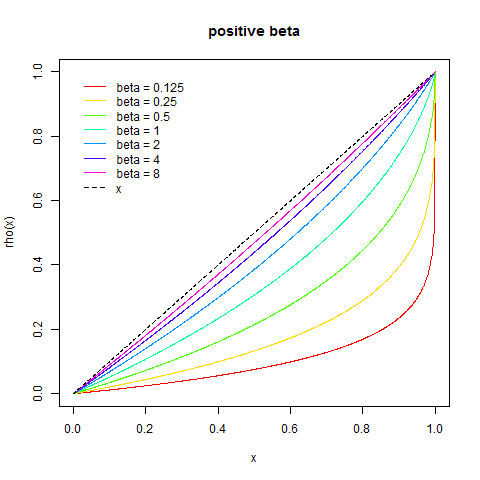
\includegraphics[width=0.7\textwidth]{fig/yule-beta.png}
	\end{center}
	\caption{Yule過程の解}\label{fig:Yule過程の解}
\end{figure} %}


\begin{todo}[今後の予定]\label{todo:今後の予定} %{
	ジーナスの確率分布$\rho(t,x)$ではなく分布そのもの$\nu(t,x)$を扱うことが
	できないだろうか?
	\EOP
\end{todo} %todo:今後の予定}
\subsection{微分方程式の解}\label{s2:微分方程式の解} %{
微分方程式\eqref{eq:diff-rho}をもう少し詳しく見る。

\subsubsection{線形の微分方程式}\label{s3:線形の微分方程式} %{
ゲージ変換を明示するために$\fukuso\pplr{x}$係数の$N$次元ベクトルで考える。

行列$A(x)\in M_N\plra{\fukuso\pplr{x}}$とベクトル$F(x)\in \fukuso\pplr{x}^N$
を固定して、次の微分方程式を考える。
\begin{equation*}\label{eq:diff-gen}
	\clD_A\phi(x) = F(x)
	\quad\text{where}\quad \clD_A\psi(x) := \plrg{\partial_x + A(x)}\psi(x)
	\quad\text{for all } \psi(x)\in\fukuso\pplr{x}^N
\end{equation*}
任意の$U(x)\in \GL_N\plra{\fukuso\pplr{x}}$と$\phi\in\fukuso\pplr{x}^N$に
対して次のゲージ変換が成り立つ。
\begin{equation*}
	\clD_A\phi(x) = \clD_AUU^{-1}\phi(x) = U\clD_{\clD_AU}U^{-1}\phi(x)
\end{equation*}
ここで、$\clD_AU$は次のように定義する。
\begin{equation*}
	\clD_AU(x) := U^{-1}(x)\plrg{\partial_x + A(x)}U(x)
	\quad\text{for all } U(x)\in \GL_N\plra{\fukuso\pplr{x}}
\end{equation*}
したがって、$D_AG=0$となる$G(x)\in \GL_N\plra{\fukuso\pplr{x}}$が求まると、
微分方程式\eqref{eq:diff-gen}の解$\phi$が次のように求まる。
\begin{equation*}
	\phi(x, y) = G(x)\int_y^x dz G^{-1}(z)F(z)
	\implies \plrgg{\partial_x + A(x)}\phi(x, y) = F(x)
\end{equation*}
そのような$G$があれば、次の式が成り立つ。
\begin{equation*}
	D_AG(x) = 0 \iff 
	A(x) = - \plrg{\partial_xG(x)}G^{-1}(x) = G(x)\partial_xG^{-1}(x)
\end{equation*}
$N=1$の場合は、ある$0<r\in\jitu$があって、$A(x)$が$\Ballx{x_0}{r}$で正則で
あれば、任意の$x\in\Ballx{x_0}{r}$に対して次のように書ける。
\begin{equation*}
	G(x) := G(x, x_0) = \exp\plra{- \int_{x_0}^x dzA(z)}
	\quad\text{for all } x\in\Ballx{x_0}{r}
	\quad\text{when } N = 1 
\end{equation*}
%s3:線形の微分方程式}
\subsubsection{微分方程式の解}\label{s3:微分方程式の解} %{
微分方程式\eqref{eq:diff-rho}を前節\ref{s3:線形の微分方程式}の筋書きに添って
解く。

\eqref{eq:diff-rho}を次のように書き直す。
\begin{equation}\label{eq:diff-rho-1}
	D_\beta\rho(x) = \frac{\beta}{1 - x} \quad\text{where}\quad
	D_\beta\phi(x) := \plrgg{\partial_x + \frac{\beta}{x(1 - x)}}\phi(x)
	\quad\text{for all } \phi(x)\in\fukuso\pplr{x}
\end{equation}
ゲージ場の積分は次のようになり、
\begin{equation*}
	\int_{x_0}^x \frac{\beta dz}{z(1 - z)}
	= \beta\ln\plra{\frac{x}{x_0}\frac{1 - x_0}{1 - x}}
	= \beta\ln\frac{\sigma(x)}{\sigma(x_0)}
\end{equation*}
ゲージ場は次のように書ける。
\begin{equation*}
	\frac{\beta}{x(1 - x)} = \sigma(x)^{-\beta}\partial_x\sigma(x)^\beta
	= \beta\partial_x\ln\sigma(x)
\end{equation*}
ここで、$\sigma$は$(0,1,\infty)$を$(0,\infty,-1)$に移すM\"obius変換で、
次のように定義する。
\begin{equation*}
	\sigma(x) := \frac{x}{1 - x}
\end{equation*}
$\sigma(x)^\beta$は、$x=0$に$\beta$次のゼロ点、$x=1$に$\beta$次の発散点を
持つ。このことは、$D_\beta$の特異点が、確定特異点の$\set{0,1}$だけに
なっていることを反映している。微分方程式\eqref{eq:diff-rho-1}の右辺は、
$\sigma$を用いて次のように書けることに注意すると、
\begin{equation*}
	\frac{\beta}{1 - x} = x\sigma(x)^{-\beta}\partial_x\sigma(x)^\beta
\end{equation*}
\eqref{eq:diff-rho-1}の解$\rho(x,y|\beta)$は次のように書ける。
\begin{equation*}
	\rho(x,y|\beta) := \sigma(x)^{-\beta}\int_y^x d\plra{\sigma(z)^\beta}z
	:= \sigma(x)^{-\beta}\int_y^x dz \plra{\partial_z\sigma(z)^\beta}z
\end{equation*}
任意の$0<\beta$に対して$x=0$で正則となることを要請すると、積分の始点$y$が
$0$に定まる。
\begin{equation}\label{eq:rho-int-1}
	\rho(x|\beta) := \rho(x,0|\beta)
	= \sigma(x)^{-\beta}\int_0^x d\plra{\sigma(z)^\beta}z
\end{equation}
この解は次の性質を満たす。

\begin{description}\setlength{\itemsep}{-1mm} %{
	\item[ベータ関数] 任意の$x\in\jitu$に対して$\rho(x|0)=0$だから、
	$0<\beta$の場合を考える。この時、\eqref{eq:rho-int-1}の積分変数を
	次のように変換していく。
	\begin{alignat*}{2}
		\rho(x|\beta) 
		&= \sigma(x)^{-\beta}\int_0^{\sigma(x)} d\plra{s^\beta} \sigma^{-1}(s)
		&\quad&\text{// } s = \sigma(z),\;\sigma^{-1}(s) = \frac{s}{1 + s} \\
		&= \int_0^1 d\plra{t^\beta} \sigma^{-1}\plrg{\sigma(x)t}
		&\quad&\text{// } t = \frac{s}{\sigma(x)} \\
		&= \beta x\int_0^1 dt \frac{t^\beta}{1 - x(1 - t)}
	\end{alignat*}
	この式では$\rho(x|0)=0$となるから、$\beta=0$の時も成り立つ。
	\begin{equation}\label{eq:rho-int-beta}
		\rho(x|\beta) = \beta x\int_0^1 dt \frac{t^\beta}{1 - x(1 - t)}
		\quad\text{for all } |x| < 1,\; 0 \le \beta
	\end{equation}
	%
	\item[級数展開] M\"obius変換を明示的に示す級数展開を導く。
	\eqref{eq:rho-int-1}の積分変数を次のように変換する。
	\begin{alignat*}{2}
		\rho(x|\beta) 
		&= \sigma(x)^{-\beta}\int_0^{\sigma(x)} d(s^\beta)\sigma^{-1}(s)
		&\quad&\text{// } s = \sigma(z),\;\sigma^{-1}(s) = \frac{s}{1 + s} \\
		&= \sigma(x)^{-\beta}\int_0^{\sigma(x)^\beta} dt\sigma^{-1}(t^{\frac{1}{\beta}})
		&\quad&\text{// } t = s^\beta
	\end{alignat*}
	$\sigma^{-1}(t^{1/\beta})$を$t^{1/\beta}=0$近傍でべき展開するが、$x$の値に
	よって場合分けする必要がある。
	\begin{description}\setlength{\itemsep}{-1mm} %{
		\item[$x\le 1/2$の時] この時は、$\sigma(x)\le 1$となり、被積分変数$t$が
		$|t|<1$となり、次のようにべき展開できる。
		\begin{equation*}
			\rho(x|\beta) = \sigma(x)^{-\beta}\int_0^{\sigma(x)^\beta} dt 
				t^{\frac{1}{\beta}}\sum_{n\in\sizen} \plra{- t^{\frac{1}{\beta}}}
			= \beta \sum_{n\in\sizen} (-)^n\frac{\sigma(x)^{n + 1}}{\beta + n + 1}
		\end{equation*}
		%
		\item[$1/2< x$の時] この時は、$1<\sigma(x)$となり、被積分変数$t$が
		$|t|<1$ではなくなり、積分範囲を分割する必要がある。
		\begin{equation*}\begin{split}
			\rho(x|\beta) 
			= \sigma(x)^{-\beta}\plra{\int_0^1 + \int_1^{\sigma(x)^\beta}} dt 
			\sigma^{-1}\plra{t^{\frac{1}{\beta}}}
		\end{split}\end{equation*}
		一つ目の積分は$x\le1/2$の場合と同じだが、二つ目の積分はべき展開が異なる。
		\begin{equation*}\begin{split}
			\sigma(x)^{-\beta}\int_1^{\sigma(x)^\beta}dt
				\sigma^{-1}\plra{t^{\frac{1}{\beta}}}
			&= \sigma(x)^{-\beta}\int_1^{\sigma(x)^\beta}dt
				\sum_{n\in\sizen}\plra{- t^{- \frac{1}{\beta}}}^n \\
			&= - \beta\sum_{n\in\sizen}(-)^n
				\frac{\sigma(x)^{- \beta} - \sigma(x)^{- n}}{\beta - n}
		\end{split}\end{equation*}
		$\beta\in\sizen$の場合、和の中に不定な項が現れるが、それは次の極限を
		とるものとする。
		\begin{equation*}
			\lim_{\beta\to n}\frac{\sigma(x)^{- \beta} - \sigma(x)^{- n}}{\beta - n}
			= - \lim_{\beta\to n}\sigma(x)^{- \beta}\ln\sigma(x)
			= - \frac{\ln\sigma(x)}{\sigma(x)^n}
		\end{equation*}
	\end{description} %}
	以上をまとめると、次の級数展開が得られる。
	\begin{equation}\label{eq:rho-int-mobius}
		\rho(x|\beta) = \beta\sum_{n\in\sizen}(-)^n\begin{cases}
			\cfrac{\sigma(x)^{n + 1}}{\beta + n + 1}
			, &\text{ if } |x| < \frac{1}{2} \\
			\cfrac{1}{\beta + n + 1} 
			- \cfrac{\sigma(x)^{- \beta} - \sigma(x)^{- n}}{\beta - n}
			, &\text{ otherwise } \\
		\end{cases}
	\end{equation}
	%
	\item[$0$の近傍] $B(1,\beta + 1)=1/(\beta + 1)$だから、次の式が成り立つ。
	\begin{equation*}
		\rho(x|\beta) = \frac{\beta}{\beta + 1}x + \bigO x^2
		\quad\text{for all } |x| < 1 ,\; 0 \le \beta
	\end{equation*}
	%
	\item[$1$の近傍] 任意の$x\in\jitu$に対して$\rho(x|0)=0$だから、
	$0<\beta$の場合を考える。この時、\eqref{eq:rho-int-beta}から、次の式が
	成り立つ。
	\begin{equation*}
		\rho(1|\beta) = \beta\int_0^1 dt t^{\beta - 1} = 1
		\quad\text{for all } 0 < \beta
	\end{equation*}
	$0<\beta$として、$\rho(x|\beta)$を微分することで1次の項を求める。
	\begin{equation*}
		\partial_x\rho(x|\beta) = \beta\int_0^1 dt \frac{t^\beta}{1 - x(1 - t)}
		+ \beta x\int_0^1 dt \frac{t^\beta(1 - t)}{\plrg{1 - x(1 - t)}^2}
	\end{equation*}
	この式で、$x\to1$の極限をとると、一項目は任意の$0<\beta$で$1$になるが、
	二項目は$\beta\le1$で発散する。
	\begin{equation*}
		\lim_{x\to1} x\int_0^1 dt \frac{t^\beta(1 - t)}{\plrg{1 - x(1 - t)}^2}
		= \begin{cases}
			B(\beta - 1, 2), &\text{ iff } 1 < \beta \\
			\infty, &\text{ otherwise } \\
		\end{cases}
	\end{equation*}
	$\beta\le1$の場合は、$x=1$で微分不可能になり、次の式が成り立つ。
	\begin{equation*}
		\lim_{x\to1-0}\partial_x\rho(x|\beta)
		= \begin{cases}
			\cfrac{\beta}{\beta - 1}, &\text{ if } 1 < \beta \\
			\infty, &\text{ otherwise } \\
		\end{cases}
	\end{equation*}
	%
	\item[$\beta=0$の極限] $\beta=0$の時は、任意の$x\in\jitu$に対して
	$\rho(x|0)=0$となる。一方、任意の$0<\beta$で$\rho(1|\beta)=1$だから、
	$\lim_{\beta\to0+0}\rho(1|\beta)\neq\rho(1|0)$となって、$\rho(x|\beta)$は
	$\beta$について$0$で不連続になる。
	%
	\item[$\beta=\infty$の極限] 級数展開\eqref{eq:rho-int-mobius}で
	$\beta\to\infty$の極限をとると、$|x|\le1/2$の時は次のようになり、
	\begin{equation*}
		\lim_{\beta\to\infty}\rho(x|\beta)
		= \sum_{n\in\sizen}(-)^n\sigma(x)^{n+1}
		= \frac{\sigma(x)}{1 + \sigma(x)} = x
	\end{equation*}
	$1/2<x<1$の時は次のようになる。
	\begin{equation*}
		\lim_{\beta\to\infty}\rho(x|\beta)
		= \sum_{n\in\sizen}(-)^n\sigma(x)^{-n}
		= \frac{\sigma(x)}{1 + \sigma(x)} = x
	\end{equation*}
	したがって、任意の$0<\beta$で$\rho(x|\beta)=1$だから、次の式が成り立つこと
	がわかる。
	\begin{equation*}
		\lim_{\beta\to\infty}\rho(x|\beta) = x \quad\text{for all } 0\le x\le 1
	\end{equation*}
\end{description} %}
%s3:微分方程式の解}

\section{計算}\label{s1:計算} %{
\subsection{ベータ関数}\label{s2:ベータ関数} %{
$0<\Re x,\; 0<\Re y$に対してベータ関数$B(x,y)$は次のように定義される。
\begin{equation}\label{eq:Beta}
	B(x, y) := \int_0^1\frac{dt}{t(1-t)}t^x(1-t)^y
	\quad\text{for all } 0<\Re x,\; 0<\Re y
\end{equation}

ベータ関数とガンマ関数は次の関係にある。
\begin{equation}
	B(x, y) = \frac{\Gamma(x)\Gamma(y)}{\Gamma(x+y)}
	\quad\text{for all } 0<\Re x,\; 0<\Re y
\end{equation}
\begin{proof} %{
	定義\eqref{eq:Beta}の積分変数を$s:=t/(1-t)$と変換すると、ガンマ関数の
	積分表示が現れる。
	\begin{alignat*}{2}
		B(x, y) &= \int_0^\infty\frac{ds}{s}\frac{s^x}{(1+s)^{x+y}}
		&\quad&\text{// } s := \frac{t}{1-t} \\
		&= \frac{1}{\Gamma(x+y)}\int_0^\infty\frac{ds}{s}s^x
		\int_0^\infty\frac{du}{u}u^{x+y}e^{-(1+s)u}
		&\quad&\text{// } \Gamma(x) = a^x\int_0^\infty\frac{dt}{t}t^xe^{-at} \\
		&= \frac{1}{\Gamma(x+y)}\int_0^\infty\frac{du}{u}u^{x+y}e^{-u}
		\int_0^\infty\frac{ds}{s}s^xe^{-su} \\
		&= \frac{\Gamma(x)}{\Gamma(x+y)}\int_0^\infty\frac{du}{u}u^ye^{-u} \\
		&= \frac{\Gamma(x)\Gamma(y)}{\Gamma(x+y)}
	\end{alignat*}
\end{proof} %}

定義\eqref{eq:Beta}の積分路を変形して、$y$の実部が負の場合に解析接続しよう。
$C$を図\ref{fig:ベータ関数の積分路その一}の積分路とすると、次の式が成り立つ。
\begin{equation*}
	B(x,y) = \frac{1}{1 - e^{-2\pi iy}}\int_C \frac{dt}{t(1 - t)}t^x(1 - t)^y
	\quad\text{for all } 0 < \Re x,\; 0 < \Re y,\; y\not\in\sei
\end{equation*}
ここで、複素平面の分岐切断は、$x\in\sei$の時は$(-\infty,1)$、$x\not\in\sei$
の時は$(0,1)$とする。

\begin{figure}[htbp] %{
	\begin{center}
		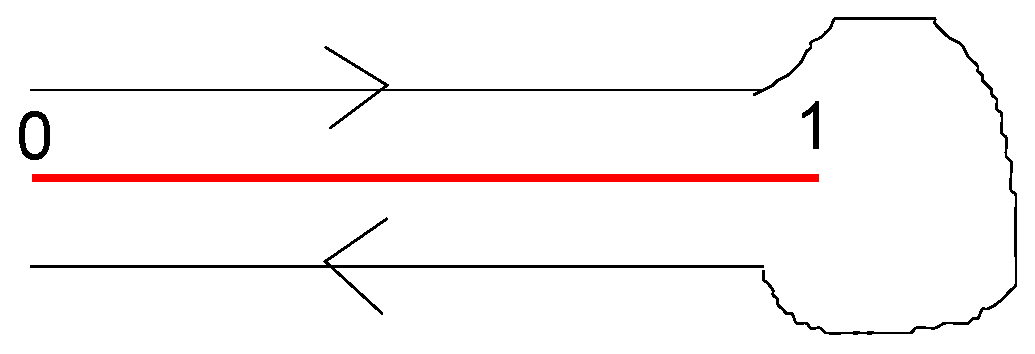
\includegraphics[width=0.3\textwidth]{fig/contour-2.eps}
	\end{center}
	\caption{ベータ関数の積分路その一}\label{fig:ベータ関数の積分路その一}
\end{figure} %}
%s2:ベータ関数}
\subsection{ベータ関数の和}\label{s2:ベータ関数の和} %{
$0<\Re a$かつ$0<\Re b$とすると、次の式が成り立ち、
\begin{equation*}
	\sum_{n\in\sizen}B(n + a, b)x^n = \int_0^1 frac{dt}{t(1 - t)}t^a(1 - t)^b 
		\sum_{n\in\sizen}(tx)^n
	= \int_0^1 \frac{dt}{t(1 - t)}\frac{t^a(1 - t)^b}{1 - xt}
\end{equation*}
次の式が得られる。
\begin{equation*}\begin{split}
	\sum_{n\in\sizen}B(n + a, b) = B(a, b - 1) 
\end{split}\end{equation*}
%s2:ベータ関数の和}
\subsection{二項係数の計算}\label{s2:二項係数の計算} %{
任意の$0<k\in\jitu,\;x\in\Ballx{0}{1}$に対して次の式が成り立つ。
\begin{equation}\label{eq:分数の二項係数}
	(1 - x)^{-k} = \sum_{n\in\sizen}\frac{x^n\Gamma(k+n)}{n!\Gamma(k)}
	= \sum_{n\in\sizen}\frac{x^n}{(n + k)B(n + 1, k)}
\end{equation}
$k\in\fukuso$でも成り立つと思うが、その場合は解析接続が必要になる。
%s2:二項係数の計算}
%s1:計算}

\section{バックアップ}\label{s1:バックアップ} %{
\subsection{分岐を持つ複素積分} % (fold)
\label{sub:分岐を持つ複素積分}
単位円上の積分$\oint_{|z|=1}dzz^{\frac{1}{2}}$を考える。
円座標を使って計算すると次のようになる。
\begin{alignat*}{2}
	\oint_{|z|=1}dzz^{\frac{1}{2}}
	&= i\int_0^{2\pi} d\theta \exp\plra{\frac{3i}{2}\theta}
	&\quad&\text{// } z = \exp\plra{i\theta} \\
	&= \frac{2}{3}\blra{\exp\plra{\frac{3i}{2}\theta}}_{\theta=0}^{2\pi}
	= - \frac{4}{3}
\end{alignat*}
積分路の組み合わせを使って計算してみよう。図\ref{fig:積分路その一}のように、
$C_1$を$|z|=1$の反時計回りの円周、$C_\epsilon$を$|z|=\epsilon<1$の時計回りの円周、
$L_+$を$\epsilon$から$1$への実軸上の直線、$L_-$を$1$から$\epsilon$への実軸上の直線とし、
それらを繋げた閉路を$\Gamma$とする。
\begin{equation*}
	\oint_\Gamma = \int_{C_1} + \int_{L_-} + \int_{C_\epsilon} + \int_{L_+}
\end{equation*}
$dzz^{\frac{1}{2}}$の分岐を正の実軸にとると、$\Gamma$の内部には$dzz^{\frac{1}{2}}$の極と
分岐が無いので、$\oint_\Gamma dzz^{\frac{1}{2}}=0$となり、
$\lim_{\epsilon\to0}\int_{C_\epsilon}dzz^{\frac{1}{2}}=0$だから、次の式が成り立つ。
\begin{equation}\begin{split}\label{eq:branch-1}
	\int_{C_1}dzz^{\frac{1}{2}} 
	&= - \lim_{\epsilon\to0}\plra{\int_{L_-} + \int_{L_+}}dzz^{\frac{1}{2}} \\
	&= - \int_1^0 dze^{\pi i}z^{\frac{1}{2}} - \int_0^1 dzz^{\frac{1}{2}}
	= \int_1^0 dzz^{\frac{1}{2}} - \int_0^1 dzz^{\frac{1}{2}} = - \frac{4}{3}
\end{split}\end{equation}

\begin{figure}[htbp] %{
	\begin{center}
		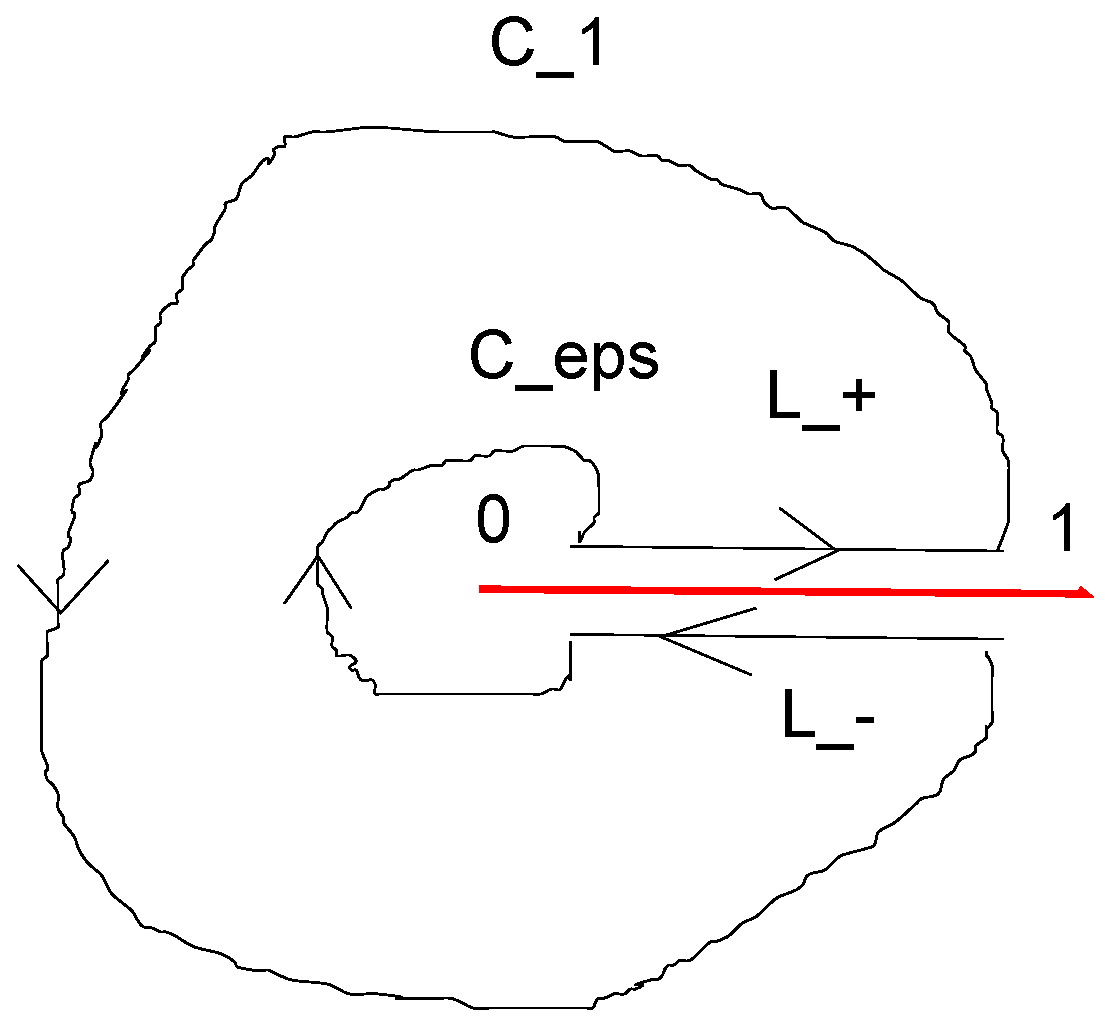
\includegraphics[width=0.3\textwidth]{fig/contour-1.eps}
	\end{center}
	\caption{積分路その一}\label{fig:積分路その一}
\end{figure} %}

$\int_1^z$の積分路によって$\ln z$の多意性$\ln z+2n\pi i$を表すことができる。
積分路が原点の周りを時計回りに一周する毎に、$2\pi i$ずつ$\ln z$に加算されて
いく。逆に、多意性を取り除くために、複素平面から原点を取り除き、原点から
無限遠点までハサミで切断した空間$K_0$を考え、$\int_1^z$の積分路を$K_0$内に
限定したものを$\ln z$と定義し、$z^a$を$e^{a\ln z}$によって定義する。
\eqref{eq:branch-1}の$L_-$による積分の被積分関数の因子$e^{\pi i}$は、
正の実軸を分岐切断として計算されたものになっている。

\cite{hb3.s6:online}\cite{www.e5:online}はリーマン面の簡潔な
イントロダクションだと思う。\cite{www.s3:online}は超幾何関数について古典的
な結果とそれを現代的な視点で捉え直したところまで網羅した概観を与えている。
% subsection 分岐を持つ複素積分 (end)
%s1:バックアップ}

\bibliographystyle{jplain}
\bibliography{local}
\end{document}
